%%%%%%%%%%%%%%%%%%%%%%%%%%%%%%%%%%%%%%%%%
% Programming/Coding Assignment
% LaTeX Template
%
% This template has been downloaded from:
% http://www.latextemplates.com
%
% Original author:
% Ted Pavlic (http://www.tedpavlic.com)
%
% Note:
% The \lipsum[#] commands throughout this template generate dummy text
% to fill the template out. These commands should all be removed when 
% writing assignment content.
%
% This template uses a Perl script as an example snippet of code, most other
% languages are also usable. Configure them in the "CODE INCLUSION 
% CONFIGURATION" section.
%
%%%%%%%%%%%%%%%%%%%%%%%%%%%%%%%%%%%%%%%%%

%----------------------------------------------------------------------------------------
%	PACKAGES AND OTHER DOCUMENT CONFIGURATIONS
%----------------------------------------------------------------------------------------

\documentclass{article}

\usepackage{fancyhdr} % Required for custom headers
\usepackage{lastpage} % Required to determine the last page for the footer
\usepackage{extramarks} % Required for headers and footers
\usepackage[usenames,dvipsnames]{color} % Required for custom colors
\usepackage{graphicx} % Required to insert images
\usepackage{listings} % Required for insertion of code
\usepackage{courier} % Required for the courier font
\usepackage{lipsum} % Used for inserting dummy 'Lorem ipsum' text into the template
\usepackage[utf8]{inputenc} % Required for inputting international characters
\usepackage[T1]{fontenc} % Output font encoding for international characters
\usepackage{pdfpages}

% Margins
\topmargin=-0.45in
\evensidemargin=0in
\oddsidemargin=0in
\textwidth=6.5in
\textheight=9.0in
\headsep=0.25in

\linespread{1.1} % Line spacing

% Set up the header and footer
\pagestyle{fancy}
\lhead{\hmwkTitle} % Top left header
\rhead{\hmwkAuthorName} % Top right header
%\chead{\hmwkClass\ (\hmwkClassInstructor\ \hmwkClassTime): \hmwkTitle} % Top center head
%\rhead{\firstxmark} % Top right header
\lfoot{\lastxmark} % Bottom left footer
\cfoot{} % Bottom center footer
\rfoot{Strana\ \thepage\ - \protect\pageref{LastPage}} % Bottom right footer
\renewcommand\headrulewidth{0.4pt} % Size of the header rule
\renewcommand\footrulewidth{0.4pt} % Size of the footer rule

\setlength\parindent{30pt} % potentially removes all indentation from paragraphs

%----------------------------------------------------------------------------------------
%	CODE INCLUSION CONFIGURATION
%----------------------------------------------------------------------------------------

\definecolor{MyDarkGreen}{rgb}{0.0,0.4,0.0} % This is the color used for comments
\lstloadlanguages{C++} % Load C++ syntax for listings
\lstset{language=C++, % Use c++ in this example
        frame=single, % Single frame around code
        basicstyle=\small\ttfamily, % Use small true type font
        keywordstyle=[1]\color{Blue}\bf, % c++ functions bold and blue
        keywordstyle=[2]\color{Purple}, % c++ function arguments purple
        keywordstyle=[3]\color{Blue}\underbar, % Custom functions underlined and blue
        identifierstyle=, % Nothing special about identifiers                                         
        commentstyle=\usefont{T1}{pcr}{m}{sl}\color{MyDarkGreen}\small, % Comments small dark green courier font
        stringstyle=\color{Purple}, % Strings are purple
        showstringspaces=false, % Don't put marks in string spaces
        tabsize=5, % 5 spaces per tab
        %
        % Put standard c++ functions not included in the default language here
        morekeywords={rand},
        %
        % Put c++ function parameters here
        morekeywords=[2]{on, off, interp},
        %
        % Put user defined functions here
        morekeywords=[3]{test},
       	%
        morecomment=[l][\color{Blue}]{...}, % Line continuation (...) like blue comment
        numbers=left, % Line numbers on left
        firstnumber=1, % Line numbers start with line 1
        numberstyle=\tiny\color{Blue}, % Line numbers are blue and small
        stepnumber=5 % Line numbers go in steps of 5
}

% Creates a new command to include a perl script, the first parameter is the filename of the script (without .pl), the second parameter is the caption
\newcommand{\perlscript}[2]{
\begin{itemize}
\item[]\lstinputlisting[caption=#2,label=#1]{#1.pl}
\end{itemize}
}

%----------------------------------------------------------------------------------------
%	DOCUMENT STRUCTURE COMMANDS
%	Skip this unless you know what you're doing
%----------------------------------------------------------------------------------------

% Header and footer for when a page split occurs within a problem environment
\newcommand{\enterProblemHeader}[1]{
\nobreak\extramarks{#1}{#1 pokračování na další straně\ldots}\nobreak
\nobreak\extramarks{#1 (pokračování)}{#1 pokračování na další straně\ldots}\nobreak
}

% Header and footer for when a page split occurs between problem environments
\newcommand{\exitProblemHeader}[1]{
\nobreak\extramarks{#1 (pokračování)}{#1 pokračování na další straně\ldots}\nobreak
\nobreak\extramarks{#1}{}\nobreak
}

%----------------------------------------------------------------------------------------
%	NAME AND CLASS SECTION
%----------------------------------------------------------------------------------------

\newcommand{\hmwkTitle}{Digitální model terénu a jeho analýzy} % Assignment title
\newcommand{\hmwkDueDate}{Datum odevzdání: 7.1.2018} % Due date
\newcommand{\hmwkClass}{155ADKG} % Course/class
%\newcommand{\hmwkClassTime}{10:30am} % Class/lecture time
%\newcommand{\hmwkClassInstructor}{Jones} % Teacher/lecturer
\newcommand{\hmwkAuthorName}{Petra~Millarová, ~Oleksiy~Maybrodskyy} % Your name

%----------------------------------------------------------------------------------------
%	TITLE PAGE
%----------------------------------------------------------------------------------------

\title{
\vspace{2in}
\textmd{\textbf{\hmwkClass:\ \hmwkTitle}}\\
\normalsize\vspace{0.1in}\large{\hmwkDueDate}\\
%\vspace{0.1in}\large{\textit{\hmwkClassInstructor\ \hmwkClassTime}}
\vspace{3in}
}

\author{\textbf{\hmwkAuthorName}}
\date{} % Insert date here if you want it to appear below your name

%----------------------------------------------------------------------------------------

\begin{document}

\maketitle

%----------------------------------------------------------------------------------------
%	TABLE OF CONTENTS
%----------------------------------------------------------------------------------------

%\setcounter{tocdepth}{1} % Uncomment this line if you don't want subsections listed in the ToC

\newpage
\tableofcontents
\newpage

%----------------------------------------------------------------------------------------
%	PROBLEM 1
%----------------------------------------------------------------------------------------

% To have just one problem per page, simply put a \clearpage after each problem

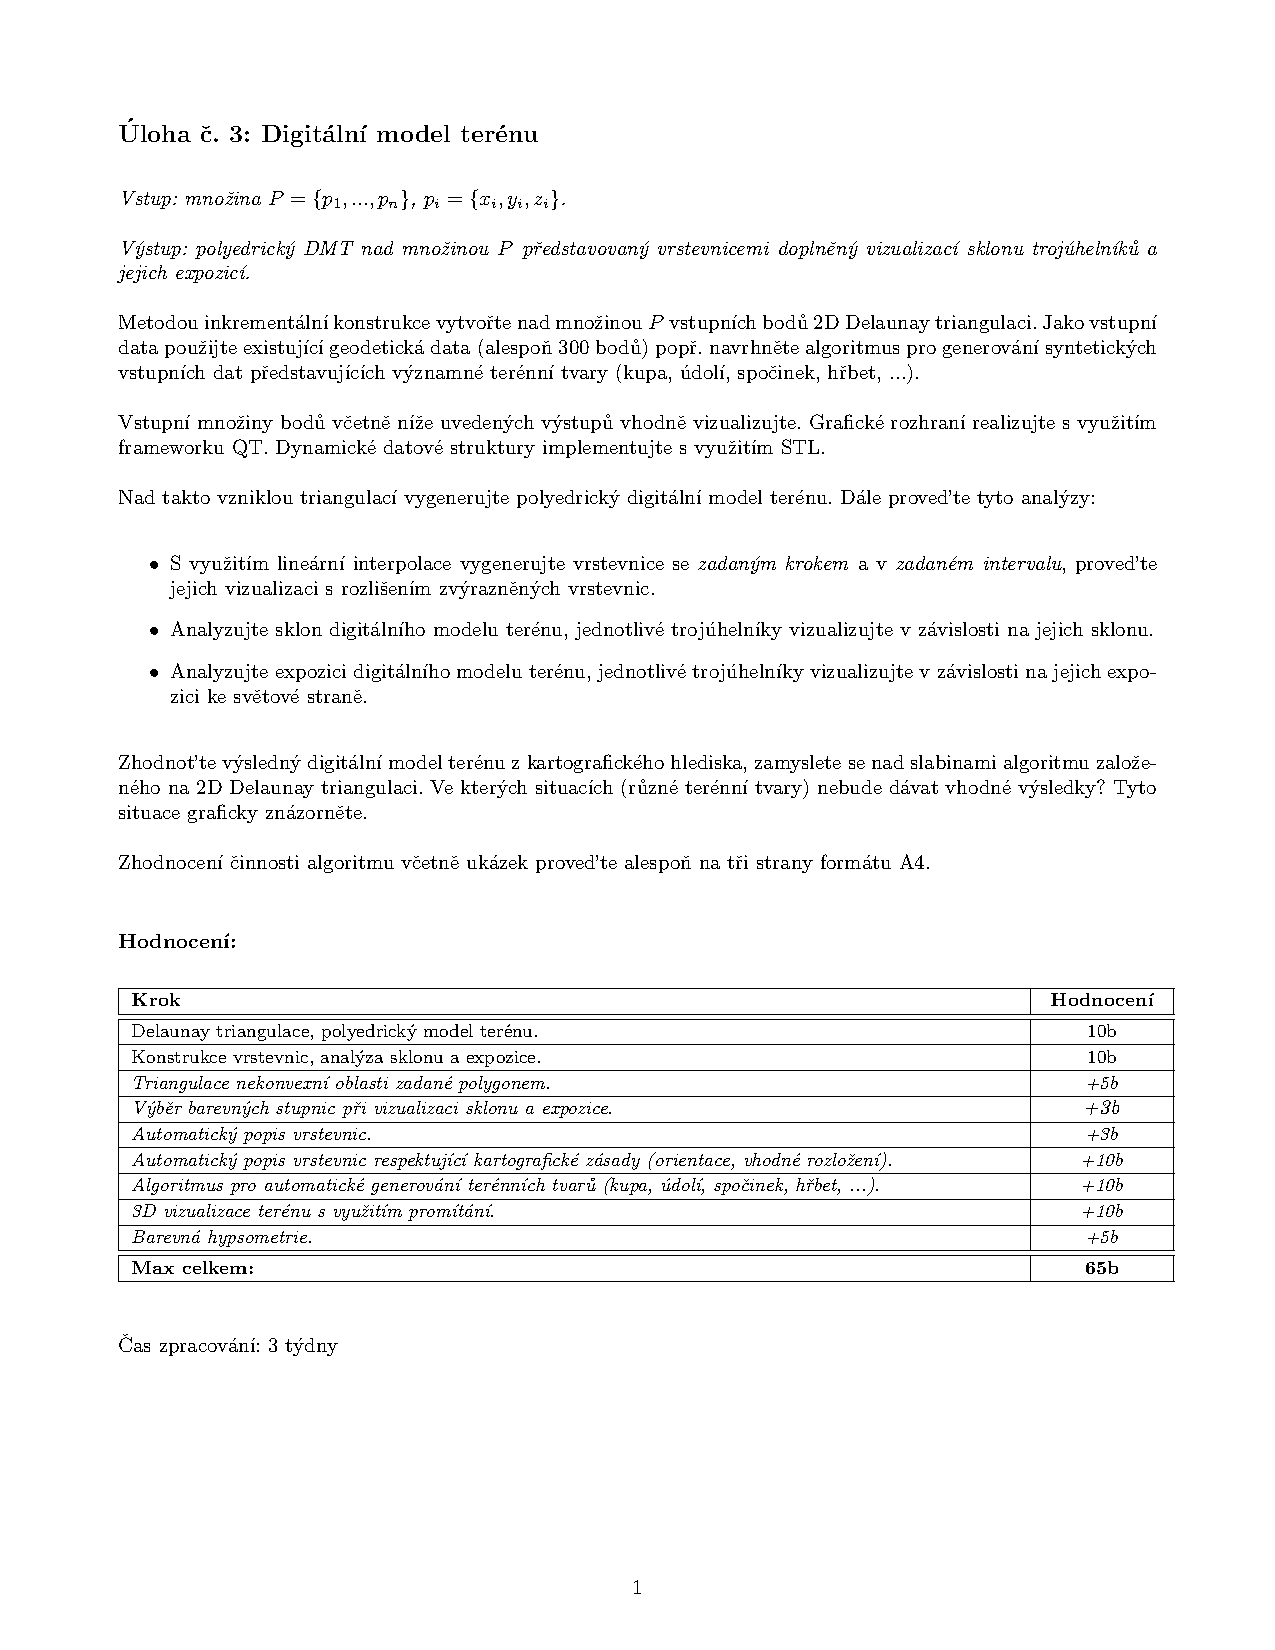
\includepdf[scale=0.9,pages=1,pagecommand=\section{Zadání}]{zadani.pdf}
\section{Popis a rozbor problému} %+vzorce
\indent Výstupem je program, který dokáže vytvořit nad prostorovou množinou DMT pomocí triangulace, vrstevnice a vizualizovat sklon terénu a jeho expozici. 

\section{Popisy algoritmů} %formálním jazykem
\subsection{Delaunay triangulace}
\indent Delaunay triangulace je nejčastěji používanou triangulací v oblasti GIS, lze jí provádět jak plošně, tak prostorově. \\
\textbf{Podmínky DLT}
\begin{itemize}
	\item Uvnitř kružnice v libovolném trojúhelníku triangulace neleží žádný jiný bod množiny.
	\item Tato triangulace maximalizuje minimální úhel v trojúhelníku, avšak neminimalizuje maximální úhel.
	\item Je lokálně i globálně optimální vůči kritériu minimálního úhlu. 
	\item Triangulace je jednoznačná, pokud žádné čtyři body neleží na kružnici.
\end{itemize}
\indent Triangulace byla realizována metodou inkrementální konstrukce. Tato metoda je založena na postupném přidávání bodů do již vytvořené triangulace. Hledá se takový bod, který má spolu s dvěma body triangulace nejmenší opsanou kružnici. Každá hrana trojúhelníku je orientována a body hledáme pouze vlevo od ní. \\
\indent Pokud je nalezen vyhovující bod, jsou do výsledné triangulace přidány orientované hrany nového trojúhelníku. Pokud neexistuje žádný takový bod, změníme orientaci hrany a hledání opakujeme. \\
\indent Pro ukládání hran se používá tzv. \textit{Active Edge List}. Tato struktura obsahuje hrany, ke kterým hledáme třetí bod. Když je třetí bod k hraně nalezen, hrana je odebrána ze seznamu. Následně se kontroluje, zda není v AEL tato hrana již přítomna s opačnou orientací. Pokud je, je z tohoto seznamu odstraněna. Pokud není, je hrana do AEL naopak přidána. V každém případě je ale hrana přidána do výsledné triangulace. Takto se v algoritmu postupuje, dokud není AEL prázdný. 
\textit{Postup při inkrementální konstrukci: }
\begin{itemize} 
\item náhodný bod \textit{$p_1$} a jemu nejbližší bod \textit{$p_2$}
\item hrana \textit{$e_1$} z bodů \textit{$p_1$} a \textit{$p_2$}
\item \textit{$p_3$} je bod s nejmenší Delaunay vzdáleností k hraně \textit{$e_1$} vlevo od hrany. 
\item pokud se žádný bod nenajde, prohodí se orientace hrany \textit{$e_1$} a hledá se znovu
\item po nalezení bodu \textit{$p_3$} se z \textit{$p_1, p_2, p_3$} vytvoří hrany \textit{$e_2$} a \textit{$e_3$} které spolu s hranou \textit{$e_1$} tvoří orientovaný trojúhelník
\item dokud není AEL prázdný, přidej \textit{$e_1, e_2, e_3$} do AEL: 
	\begin{itemize}
	\item \textit{$e_1$} první hrana AEL
	\item změna orientace \textit{$e_1$}
	\item hledáme bod \textit{p} který má nejmenší Delaunay vzdálenost vlevo od otočené \textit{$e_1$}
	\item pokud takový bod existuje, přidej \textit{$e_2, e_3$} do AEL a hranu  \textit{$e_1$} do triangulace
	\item pokud takový bod neexistuje, odstraň \textit{$e_1$} z AEL
	\end{itemize}
\end{itemize}
\subsection{Vrstevnice}
\indent Vrstevnice byly počítány pomocí lineární interpolace. U lineární interpolace je rozestup mezi dvěma body konstantní, spád terénu taktéž. \\
\indent Princip spočívá ve vyhledání průsečnice roviny určené postupně každým trojúhelníkem a roviny vodorovné se zadanou výškou \textit{h}, ve které chceme bod vrstevnice nalézt. \\
\indent Zda protíná rovina stranu trojúhelníku lze zjistit jednoduchým testem:
$(z-z_i)(z-z_{i+1}))<0$.
\indent Pokud je průsečnicí těchto rovin úsečka, vypočítají se souřadnice jejích bodů následovně:
$$ x_a = \frac{(x_3-x_1)}{z_3-z_1}(z-z_1)+x_1, $$
$$y_a = \frac{(y_3-y_1)}{z_3-z_1}(z-z_1)+y_1,$$
$$ x_b = \frac{(x_2-x_1)}{z_2-z_1}(z-z_1)+x_1, $$
$$y_b = \frac{(y_2-y_1)}{z_2-z_1}(z-z_1)+y_1.$$
\subsection{Počítání sklonu} 
\indent Výpočet sklonu se provádí nad každým trojúhelníkem v DMT. Trojúhelník je jasně daný dvěma vektory, odchylka $\varphi$ dvou rovin se spočte následovně: 
$$\varphi = \arccos(\frac{n_1n_2}{|n_1n_2|}).$$
\subsection{Orientace svahu}
\indent Orientace svahu v bodě je definována jako azimut $A$ průmětu gradientu $\bigtriangledown\rho(x_0,y_0,z_0)$ do roviny $xy$, který se spočte jako
$$A = \arctan(\frac{n_1}{n_2}), A\in\langle0,2\pi),$$
kde $n_1, n_2$ jsou vektorové součiny vektorů, které tvoří daný trojůhelník.

\section{Vstupní data}
\indent Do programu lze načíst soubor ve formátu \textit{*.txt}, který na každém řádku obsahuje XYZ souřadnice jednoho vkládaného bodu: \\
\texttt{
54625.84 23547.74 250.5 \\
54826.52 23580.78 266.7 \\
54752.66 23612.32 245.8 \\
.\\
.\\
.}
\section{Výstupní data}
\indent Program načte vstupní data a po stisku tlačítka \textit{Delaunay triangulation} vykreslí body a jejich triangulaci. Při každém vykreslení triangulace se aktualizuje šířka okna a podle té se pak body natransformují a zobrazí.
\indent Poté si uživatel může zvolit, zda chce vizualizaci vrstevnic (tlačítko \textit{Contour lines}) - zde je potřeba si nastavit požadovaný interval a rozmezí, ve kterém se vrstevnice generují (pro orientaci vidí uživatel výšku nejnižšího a nejvyššího z načtených bodů). Také lze barevně zobrazit sklon terénu (\textit{Slope}) a  jeho orientaci (\textit{Orientation}). Pro vyčištění plochy a ponechání pouze načtených bodů slouží tlačítko \textit{Clear}. \\


\section{Ukázky aplikace} %printscreen
\begin{figure}[hp]
\centering
        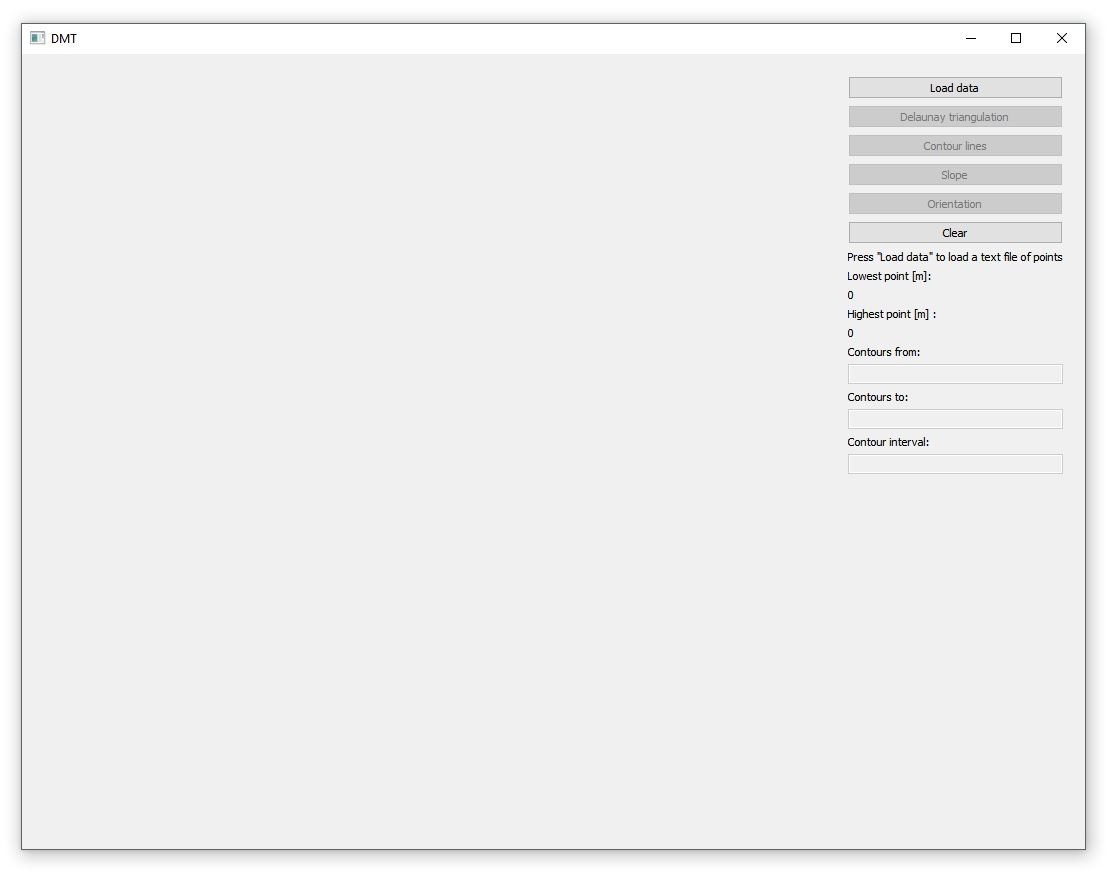
\includegraphics[trim=0cm 0cm 0cm 0cm, width=1\textwidth]{startup.jpg}
        \caption{Vzhled aplikace při otevření}
\end{figure}

\begin{figure}[hp]
\centering
        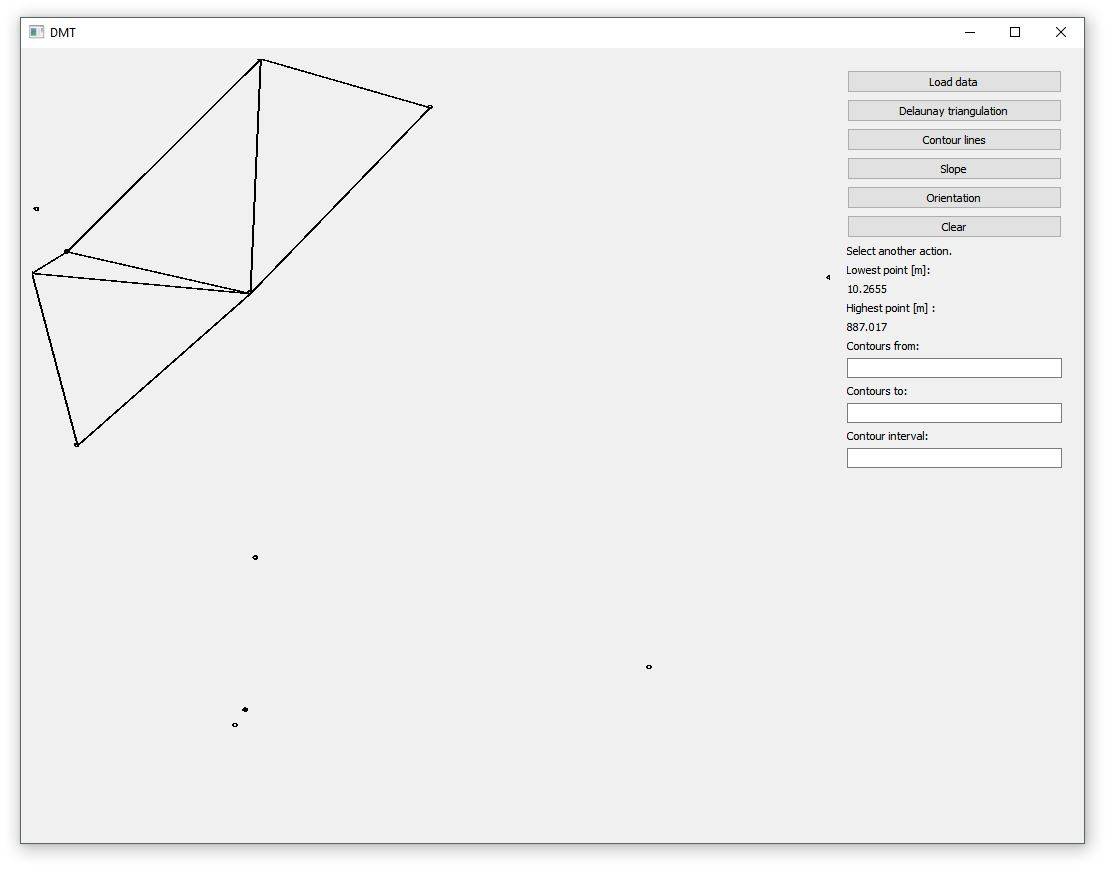
\includegraphics[trim=0cm 0cm 0cm 0cm, width=1\textwidth]{triangulate.jpg}
        \caption{Aplikace po provedení triangulace}
\end{figure}

\begin{figure}[hp]
\centering
        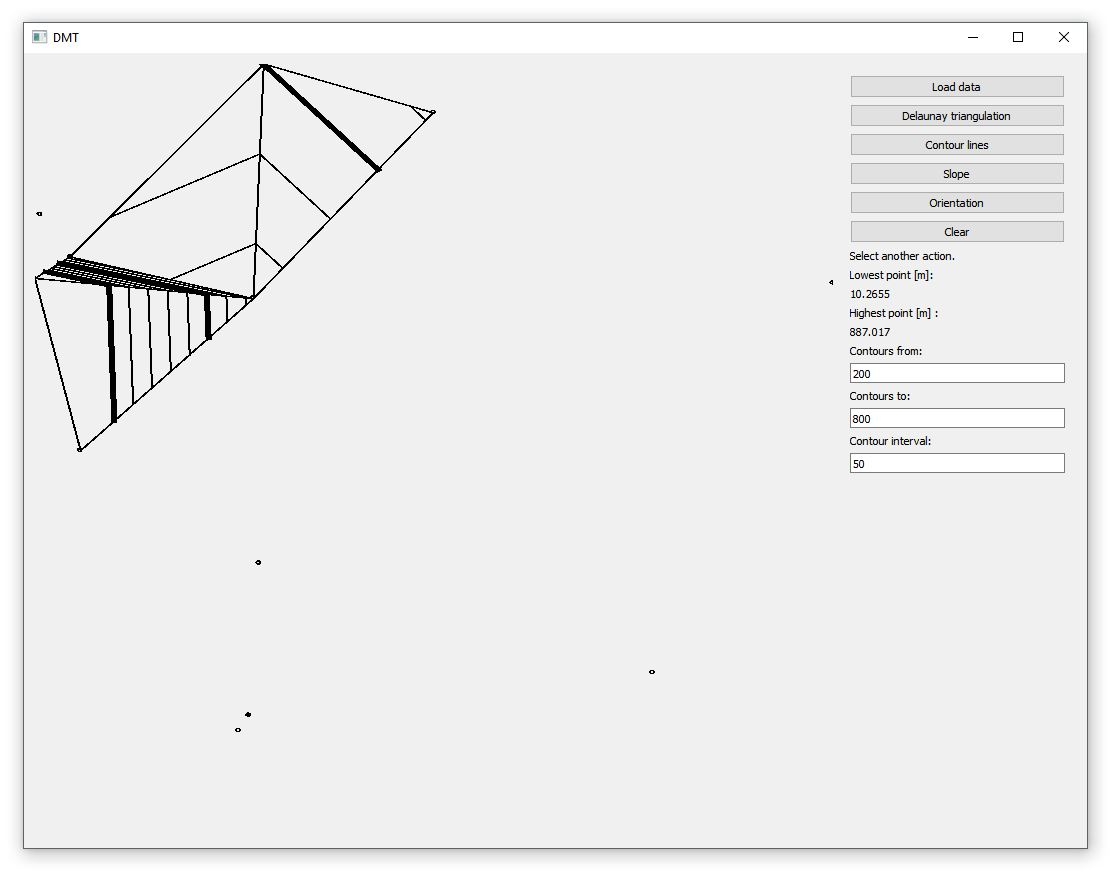
\includegraphics[trim=0cm 0cm 0cm 0cm, width=1\textwidth]{contours.jpg}
        \caption{Aplikace po zobrazení vrstevnic}
\end{figure}

\begin{figure}[hp]
\centering
        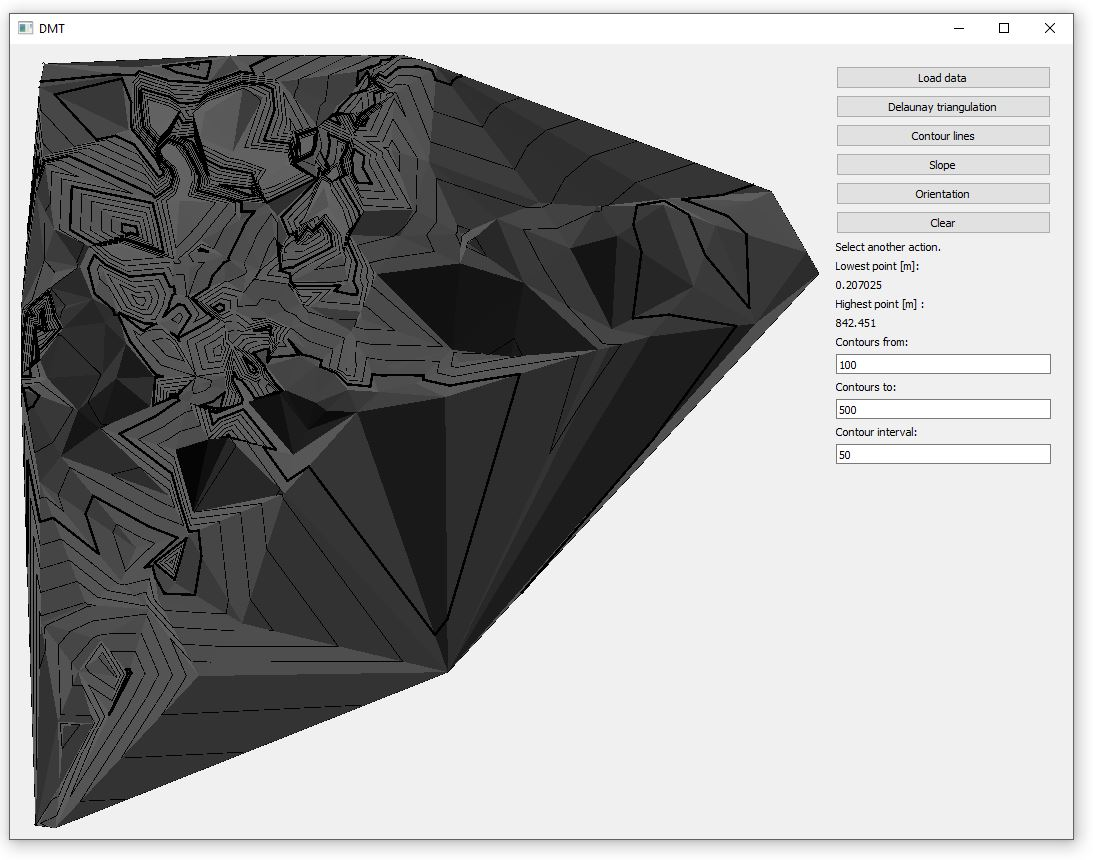
\includegraphics[trim=0cm 0cm 0cm 0cm, width=1\textwidth]{slope.jpg}
        \caption{Aplikace po vypočítání sklonu}
\end{figure}

\begin{figure}[hp]
\centering
        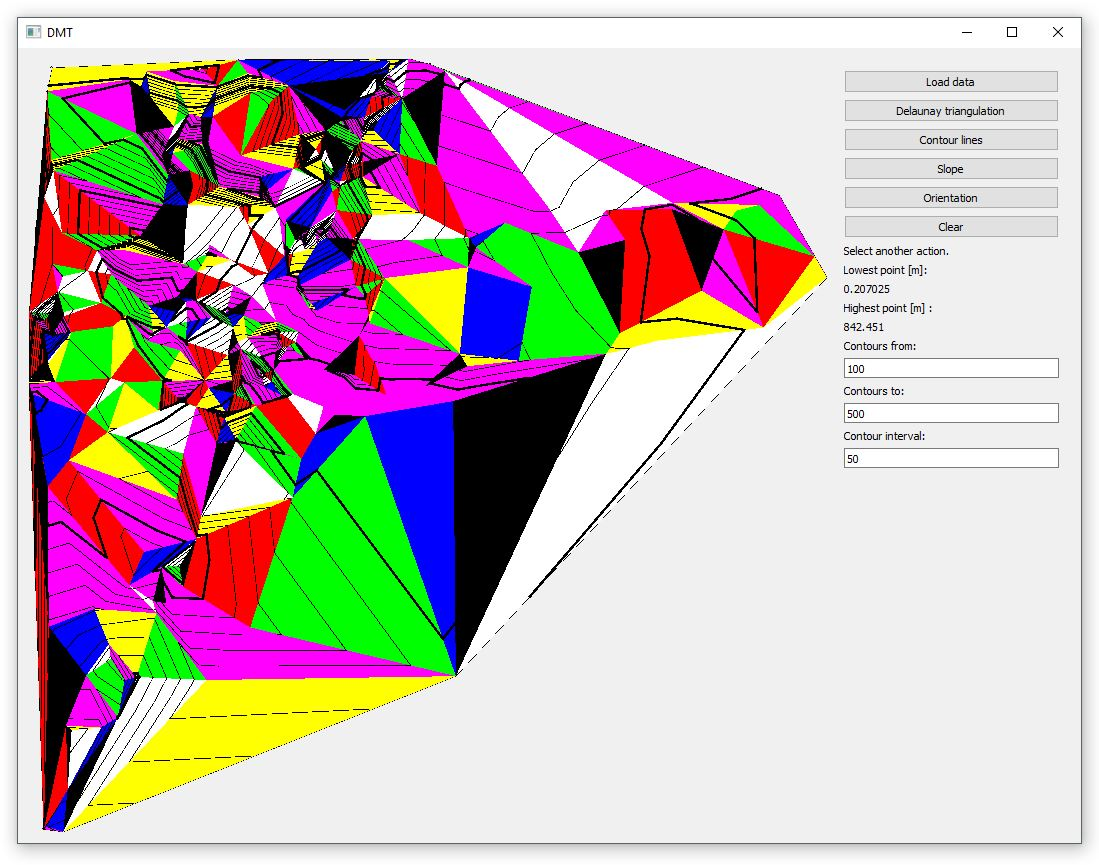
\includegraphics[trim=0cm 0cm 0cm 0cm, width=1\textwidth]{orientation.jpg}
        \caption{Aplikace po vypočtení orientace svahů}
\end{figure}

\newpage
\section{Dokumentace}

\subsubsection{Datové struktury}
\textbf{QPoint3D} - třída odvozená od třídy \textit{QPointF}, má navíc i souřadnici \textit{Z} ve formátu double. Nad třídou lze zavolat funkce \textit{getX}, \textit{getY}, \textit{getZ}, které vrací příslušnou souřadnci. \\
\textbf{Edge} - datový typ obsahující dva body typu \textit{QPoint3D}(počátek a konec hrany). Třída obsahuje přetížení operátoru \textit{==} pro porovnávání hran, funkce pro vrácení počátečního a koncového bodu hrany a funkci \textit{switchOrientation} která otáčí orientaci hrany. \\
\textbf{Triangle} je složený ze tří bodů typu \textit{QPoint3D}, svého sklonu a orientace (které jsou typu \textit{double} a implicitně nulové). Tato třída obsahuje funkce pro přístup k těmto hodnotám a funkce pro jejich pozměnění. \\

\subsubsection{Algorithms} 
 
Tato třída obsahuje algoritmy, které buď přímo slouží k výpočtům nutným pro zvládnutí této úlohy nebo jsou to algoritmy pomocné (jako např. zjištění vzájemné polohy bodu a přímky)
\bigskip
\textbf{getPosition} je funkce, která popisuje polohu bodu vůči linii. Do funkce vstupuji 3 hodnoty typu  \textbf{QPoint}, které reprezentuji dva body na přímce a bod, jehož poloha se určuje. Návratová hodnota této funkce je celé číslo \textbf{intiger}, podle výsledku testování.\\ 
 \textbf{Input:}
\begin{itemize} 
\item \textit{QPoint \&q} - testovaný bod
\item \textit{QPoint \&a} - jeden bod linie
\item \textit{QPoint \&b} - druhý bod linie
\end{itemize}
 \textbf{Output:}
\begin{itemize} 
\item 0 - bod leží vpravo od přímky
\item 1 - bod leží vlevo od přímky 
\end{itemize} 
\bigskip
\textbf{getCircleRadius} provádí výpočet poloměru kružnice zadané třemi body a výpočet středu této kružnice, jehož souřadnice se vloží do proměnné předané parametrem.\\
 \textbf{Input:}
\begin{itemize} 
\item \textit{QPoint3D \&p1} - bod kružnice
\item \textit{QPoint3D \&p2} - bod kružnice
\item \textit{QPoint3D \&p3} - bod kružnice
\item \textit{QPoint3D \&cp} - bod do kterého se vloží souřadnice středu kružnice
\end{itemize}
 \textbf{Output:}
\begin{itemize} 
\item hodnota poloměru kružnice v datovém typu \textit{double}
\end{itemize}
\bigskip
\textbf{getDelaunayPoint} hledá index takového bodu, který má od zadané hrany minimální poloměr opsané kružnice.\\
 \textbf{Input:}
\begin{itemize} 
\item \textit{Edge \&e} - hrana ke které hledáme bod
\item \textit{std::vector <QPoint3D> \&points} - vstupní množina bodů
\end{itemize}
 \textbf{Output:}
\begin{itemize} 
\item index hledaného bodu ve vektoru \textit{points}, při chybě vrací -1
\end{itemize}
\bigskip
\textbf{getNearestPoint} určuje index nejbližšího bodu k zadanému bodu
\textbf{Input:}
\begin{itemize} 
\item \textit{QPoint3D \&p} - zadaný bod
\item \textit{std::vector <QPoint3D> \&points} - vstupní množina bodů
\end{itemize}
 \textbf{Output:}
\begin{itemize} 
\item index nejbližšího bodu v datovém typu \textit{int}
\end{itemize}
\bigskip
\textbf{dt} provede vlastní triangulaci nad zadanou množinou bodů a vrací seznam orientovaných hran.
 \textbf{Input:}
\begin{itemize} 
\item \textit{std::vector <QPoint3D> \&points} - vstupní množina bodů
\end{itemize}
 \textbf{Output:}
\begin{itemize} 
\item výsledný vektor hran v datovém typu \textit{std::vector<Edge>}
\end{itemize}
\bigskip
\textbf{getConPoint} nalezne bod o zadané výšce mezi dvěma zadanými body
 \textbf{Input:}
\begin{itemize} 
\item \textit{QPoint3D \&p1} - zadaný bod
\item \textit{QPoint3D \&p2} - zadaný bod
\item \textit{double \&z} - zadaná výška
\end{itemize}
 \textbf{Output:}
\begin{itemize} 
\item bod na vrstevnici ve formátu \textit{QPoint3D}
\end{itemize}
\bigskip
\textbf{createContours} vytvoří vektor hran vrstevnic
 \textbf{Input:}
\begin{itemize} 
\item \textit{std::vector<Edge>\&dt} - triangulace na které hledáme vrstevnice
\item \textit{double zmin} - minimální výška vrstevnic
\item \textit{double zmax} - maximální výška vrstevnic
\item \textit{double h} - vzdálenost mezi vrstevnicemi
\end{itemize}
 \textbf{Output:}
\begin{itemize} 
\item seznam hran vrstevnic ve formátu \textit{std::vector<Edge>}
\end{itemize}
\bigskip
\textbf{convertDTM} převede vektor hran výsledné triangulace na vektor trojúhelíků
 \textbf{Input:}
\begin{itemize} 
\item \textit{std::vector<Edge>} - hrany výsledné triangulace
\end{itemize}
 \textbf{Output:}
\begin{itemize} 
\item \textit{std::vector<Triangle>} - převedené trojúhelníky
\end{itemize}
\bigskip
\textbf{getSlope} vypočítá sklon zadaného trojúhelníku
 \textbf{Input:}
\begin{itemize} 
\item \textit{Triangle} - zadaný trojúhelník
\end{itemize}
 \textbf{Output:}
\begin{itemize} 
\item velikost sklonu ve formátu \textit{double}
\end{itemize}
\bigskip
\textbf{getExposition} vypočítá orientaci zadaného trojúhelníku
 \textbf{Input:}
\begin{itemize} 
\item \textit{Triangle} - vstupní trojúhelník
\end{itemize}
 \textbf{Output:}
\begin{itemize} 
\item úhel natočení ve formátu \textit{double}
\end{itemize}
\textbf{getSlopes} nastavují sklony jednotlivých trojúhelníků v zadaném vektoru
 \textbf{Input:}
\begin{itemize} 
\item \textit{std::vector<Triangle> \&dtt} - vstupní vektor trojúhelníků u kterých se nastavuje sklon
\end{itemize}
 \textbf{Output:}
\begin{itemize} 
\item \textit{void}
\end{itemize}
\bigskip 

\subsubsection{Draw} 
Třída \textbf{Draw} slouží k vykreslení vypočtených triangulací, sklonů, orientací a vrstevnic.\\
\textbf{loaddata} je funkce sloužící k parsování souboru zvoleného uživatelem a vložení dat do proměnné \textit{std::vector<double> \&data}. \\

\textbf{clear}, funkce slouži k vyčištění všech dosavadních výpočtů. Ponechává pouze načtené body. \\

\textbf{delaunaydraw} vykreslí vypočtenou triangulaci. \\
\textbf{slopedraw} vykreslí sklon jednotlivých trojúhelníků triangulace. \\
\textit{orientdraw} vykreslí orientaci jednotlivých trojúhelníků triangulace. \\
\textit{countoursdrawing} vykreslí vrstevnice. \\
\textit{paintEvent} funkce volaná při každém překreslení okna, podle nastavených flags volá funkce pro vykreslení různých vlastností triangulace a triangulace samotné. \\

\subsubsection{Widget} 

Tato třída je vytvořena pro praci s grafickým rozhraním celého programu. Přes ní se provádí načtení souborů a grafické znázornění výsledků aplikace. Po kliknutí na tlačítko v aplikaci se pustí příslušná funkce v této třídě a zavolá funkci na výpočet a vykreslení, případně načtená dat.\\ 

\subsubsection{sortby-funkce}
Tyto třídní funkce slouží k seřazení vektoru souřadnic vzestupně podle velikosti buď souřadnice \textit{X} nebo \textit{Y}.

\section{Závěr a náměty na vylepšení}
Byla vytvořena aplikace, která nad Delaunay triangulací počítá a zobrazuje sklon, vrstevnice a orientaci svahu. Aplikace má pár nedostatků, které již bohužel autoři nestihli opravit. \\
\indent Samozřejmě že aplikace není bez chyb a je zde prostor pro vylepšení. Bylo by vhodné, kdyby si uživatel mohl vybrat, v odstínech jaké barvy se mu zobrazí vypočítaný sklon. Vrstevnice by mohly mít možnost popisu číslem a překreslení bodů podle velikosti okna by se mohlo provádět hned. \\
\indent Algortmus je nevhodný pro body, které jsou pravidelně rozmístěny na mřížce. Vzhledem k tomu, že triangulace funguje na principu vyhledání kružnice s nejmenším poloměrem, je pro tyto body nejednoznačná a další výpočty pak selhávají. (Viz následující obrázky)
\begin{figure}[hb]
\centering
        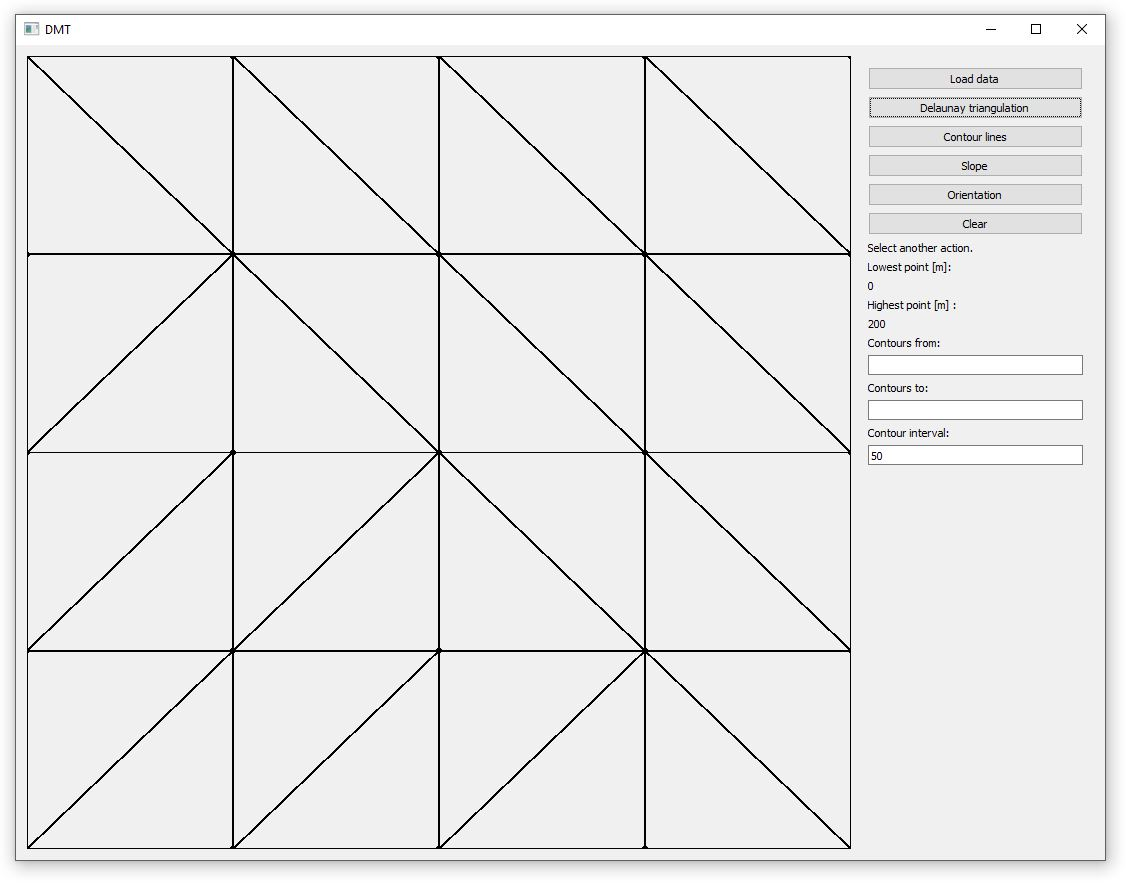
\includegraphics[trim=0cm 0cm 0cm 0cm, width=1\textwidth]{grid_dt.jpg}
        \caption{Triangulace bodů na mřížce}
\end{figure}
\begin{figure}[htb]
\centering
        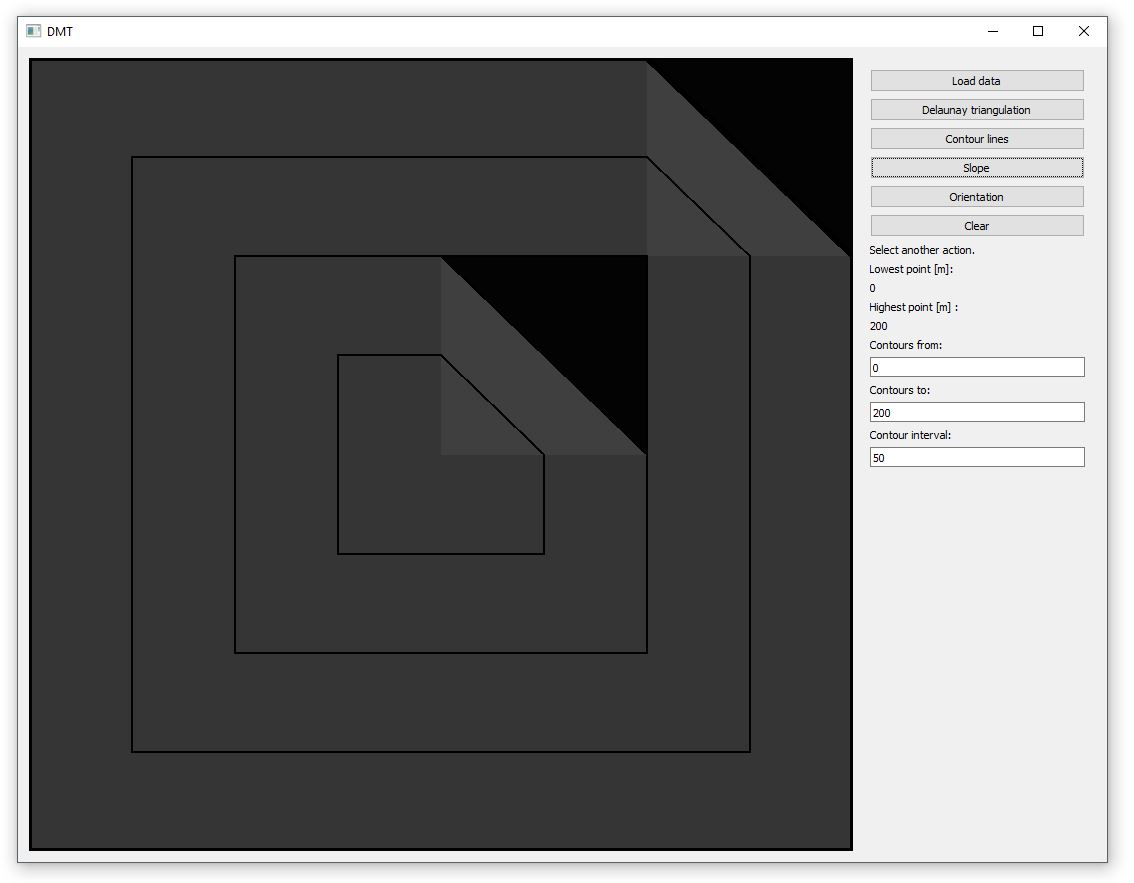
\includegraphics[trim=0cm 0cm 0cm 0cm, width=1\textwidth]{grid_slope.jpg}
        \caption{Výpočet sklonu terénu na mřížce (body ve skutečnosti tvoří pravidelný vrchol uprostřed)}
\end{figure}

	
%\pagestyle{empty}

%\end{homeworkSection}
\clearpage

%-----------------------------------------------------------------------------
\end{document}